\documentclass[sigconf]{acmart}

\usepackage{booktabs} % For formal tables

\usepackage{listings} % For SQL code
\lstset{
  basicstyle=\small\ttfamily,
  columns=flexible,
  breaklines=true,
  frame=single
}

% Copyright
\setcopyright{none}
%\setcopyright{acmcopyright}
%\setcopyright{acmlicensed}
%\setcopyright{rightsretained}

% DOI
%\acmDOI{10.475/123_4}

% ISBN
%\acmISBN{123-4567-24-567/08/06}

%Conference
\acmConference[PEARC17]{Practice \& Experience in Advanced Research Computing}{July 2017}{New Orleans, LO USA} 
\acmYear{2017}
\copyrightyear{2017}
\acmPrice{15.00}

\begin{document}
\title{Apache Airavata Sharing Service}
\subtitle{A Tool for Enabling User Collaboration in Science Gateways}

\author{Supun Nakandala}
\affiliation{
  \institution{Science Gateway Research Center}
  \institution{Indiana University}
  \city{Bloomington} 
  \state{IN}
  \country{USA} }
\email{snakanda@iu.edu}

\author{Suresh Marru}
\affiliation{
  \institution{Science Gateway Research Center}
   \institution{Indiana University}
  \city{Bloomington} 
  \state{IN}
  \country{USA} }
\email{smarru@iu.edu}

\author{Marlon Piece}
\affiliation{
  \institution{Science Gateway Research Center}
   \institution{Indiana University}
  \city{Bloomington} 
  \state{IN}
  \country{USA} }
\email{marpierc@iu.edu}

\author{Sudhakar Pamidighantam}
\affiliation{
  \institution{Science Gateway Research Center}
 \institution{Indiana University}
  \city{Bloomington} 
  \state{IN}
  \country{USA} }
\email{pamidigs@iu.edu}

\author{Kenneth Yoshimoto}
\affiliation{
  \institution{San Diego Supercomputer Center}
   \institution{University of California, San Diego}
  \city{La Jolla} 
  \state{CA}
  \country{USA} }
\email{kenneth@sdsc.edu}

\author{Terri Schwartz}
\affiliation{
  \institution{San Diego Supercomputer Center}
   \institution{University of California, San Diego}
  \city{La Jolla} 
  \state{CA}
  \country{USA} }
\email{terri@sdsc.edu}

\author{Subhashini Sivagnanam}
\affiliation{
  \institution{San Diego Supercomputer Center}
   \institution{University of California, San Diego}
  \city{La Jolla} 
  \state{CA}
  \country{USA} }
\email{sivagnan@sdsc.edu}

\author{Amit Majumdar}
\affiliation{
  \institution{San Diego Supercomputer Center}
   \institution{University of California, San Diego}
  \city{La Jolla} 
  \state{CA}
  \country{USA} }
\email{majumdar@sdsc.edu}

\author{Mark A. Miller}
\affiliation{
  \institution{San Diego Supercomputer Center}
   \institution{University of California, San Diego}
  \city{La Jolla} 
  \state{CA}
  \country{USA} }
\email{mmiller@sdsc.edu}

\begin{abstract}
Science Gateways provide user environments and a set of supporting services that help researchers make effective and enhanced use of a diverse set of computing, storage, and related resources. Gateways provide the services and tools users require  to enable their scientific exploration, which includes tasks such as running computer simulations or performing data analysis. Historically gateways have been constructed to support the workflow of individual users, but collaboration between users has become an increasingly important part of the discovery process. This trend has created a driving need for gateways to support data sharing between users. For example, a chemistry research group may want  to run simulations collaboratively, analyze experimental data or tune parameter studies based on simulation output generated by peers, whether  as a default capability, or through explicit creation of sharing privileges. As another example, students in a classroom setting may be required to share  their simulation output or data analysis results with the instructor. However most existing gateways (including the popularly used XSEDE gateways SEAGrid, Ultrascan, CIPRES, and NSG), do not support direct data sharing, so users have to handle these collaborations outside the gateway environment. Given the importance of collaboration in current scientific practice, user collaboration should be a prime consideration in building science gateways. In this work, we present design considerations and implementation of a generic model that can be used to describe and handle a diverse set of user collaboration use cases that arise in gateways, based on general requirements gathered from the SEAGrid, CIPRES, and NSG gateways. We then describe the integration of this sharing service into these gateways. Though the model and the system were tested and used in the context of Science Gateways, the concepts are universally applicable to any domain, and the service can support data sharing in a wide variety of use cases.
\end{abstract}

%
% The code below should be generated by the tool at
% http://dl.acm.org/ccs.cfm
% Please copy and paste the code instead of the example below. 
%

\begin{CCSXML}
<ccs2012>
<concept>
<concept_id>10002944.10011123.10011673</concept_id>
<concept_desc>General and reference~Design</concept_desc>
<concept_significance>500</concept_significance>
</concept>
<concept>
<concept_id>10003120.10003130.10003131.10003235</concept_id>
<concept_desc>Human-centered computing~Collaborative content creation</concept_desc>
<concept_significance>500</concept_significance>
</concept>
<concept>
<concept_id>10002951.10003227.10010926</concept_id>
<concept_desc>Information systems~Computing platforms</concept_desc>
<concept_significance>300</concept_significance>
</concept>
<concept>
<concept_id>10011007.10011074.10011134.10003559</concept_id>
<concept_desc>Software and its engineering~Open source model</concept_desc>
<concept_significance>300</concept_significance>
</concept>
</ccs2012>
\end{CCSXML}

\ccsdesc[500]{General and reference~Design}
\ccsdesc[500]{Human-centered computing~Collaborative content creation}
\ccsdesc[300]{Information systems~Computing platforms}
\ccsdesc[300]{Software and its engineering~Open source model}

\keywords{Apache Airavata, SciGaP, CIPRES, NSG, SEAGrid, Collaboration, Science Gateways, Groups, Sharing}

\maketitle

\section{Introduction}

Science gateways are science-centric user environments and supporting cyberinfrastructure that enable broader and more effective use of scientific computing resources, applications, and data \cite{gatewaySurvey2015}. Because gateways allow users to perform operations on high end resources, authentication and authorization have long been cornerstones of gateway infrastructure \cite{airavataSecurity2016},\cite{welch2007aaaa}. Authenticated access also supports another hallmark of gateways: the collection of user interactions into computational experiments that the researcher can use to monitor long running executions, retrieve results, and recall how specific results were achieved \cite{cipres2010}, \cite{seagridCommunity2016}, \cite{ultrascanAiravata2014}, \cite{nsg2013}. 
Sharing results with colleagues and making certain results publically available is the outcome of research. This is an example of user-driven authorization of something the user owns (data and metadata) rather than service provider-driven authorization of something the service provider owns (computing resources, licensed applications, etc).  Despite the fundamental nature of sharing in research, this is not a first class capability within many popular gateways. This paper examines the requirements and provides an implementation for user-directed sharing, which we apply to several popular science gateways. 
Our conceptual approach is based on group membership. Computational experiments are grouped (or tagged) into one or more organizational structures. In Apache Airavata, for example, “projects” contain experiments. These entities are by default privately owned by the creator.  The extensions are obvious: give other users and groups of users privileges to read the contents of specific experiments and groups of experiments. A subset group of these users may have additional privileges to copy, modify and execute experiments and groups of experiments. For even these simple cases, however, we know from common examples such as UNIX groups that we must reason carefully about how to implement inherited permissions, the nature of ownership and its transfer, and similar issues.

\section{Enabling collaborations within Science Gateways using Groups}

Groups are a natural choice to implement the gateway collaboration requirements outlined above. Groups themselves are just collections of entities. Entities can be  users, data collections (files, folders), resources (application software, hardware resources, quality of service), experiments. Figure 1 provides a high level architectural overview to plug in group management and sharing services to SEAGrid \cite{seagridCommunity2016}, CIPRES \cite{cipres2010} and NSG science gateways \cite{nsg2013}. Section \ref{nsg} summarizes the collaboration requirements provided by Neuroscience Gateway User Community. We summarize the sharing usecases from these gateways into 4 broad categories (Table \ref{table:usecases}). 

\begin{table}
\begin{tabular}{ |p{2cm}|p{6cm}| }
\hline
Use Case 1 & Sharing and Revoking capabilities.\\
\hline
Use Case 2 & Check Permission of a given Entity.\\
\hline
Use Case 3 & Get all accessible entities of a given user.\\
\hline
Use Case 4 & Browse and Search within all accessible entities for a given user.\\
\hline
\end{tabular}
\caption{Gateway Use cases for Collaboration}
\end{table}\label{table:usecases}

\begin{figure*}
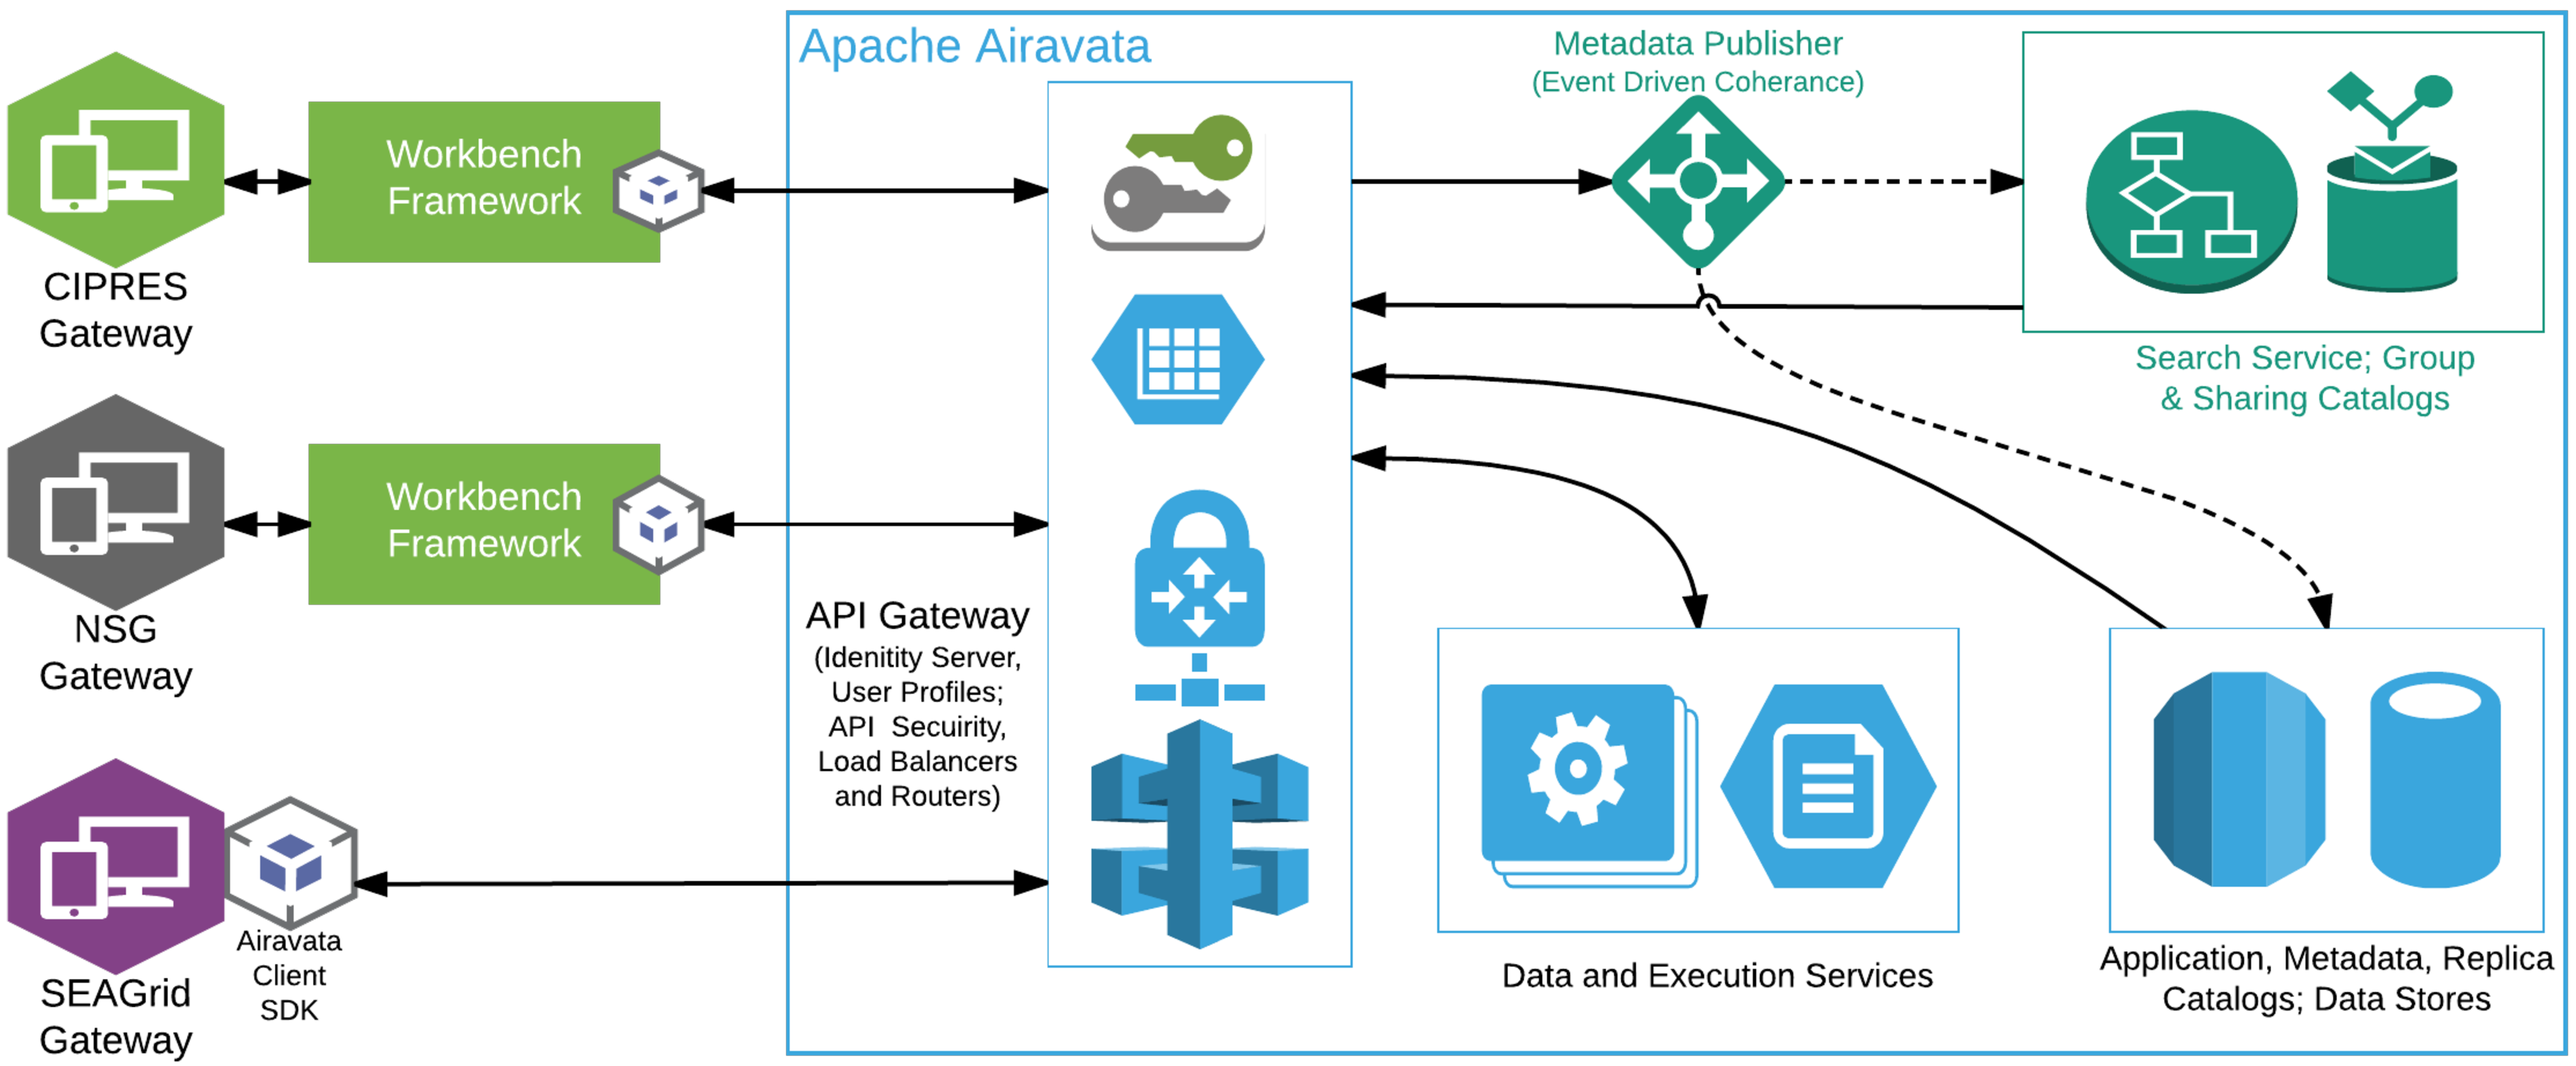
\includegraphics[height=3in, width=7in]{figures/gateway-integaration-overview.pdf}
\caption{High level architectural overview. SEAGrid Gateway is built over Apache Airavata for all data and execution capabilities; CIPRES and NSG Gateways are built over Workbench Framework and are exploring use of Apache Airavata for Data Sharing capabilities. The paper focuses on Sharing Service (green color box) and existing literature on Airavata discuss other capabilities (blue colored boxes).}
\end{figure*}

Generic implementations of groups, and “groups as a service” software exist as standalone tools and services and are integrated with common identity management software. LDAP Groups \cite{aclLDAP} and Grouper \cite{grouperWebsite} are well known examples. Grouper is a comprehensive group management software and can be deployed at university scale to manage complicated collections of users and other entities. Grouper can very well be adapted to meet the gateway Use Cases 1 and 2. But despite their power and flexibility in handling groups, the lack of flexible querying makes it not a good match for gateway Use Cases 3 and 4.

The core of the problem is that assigning an arbitrary parent-child relationship between groups does not directly express the needed permission-based relationship between the groups.  The parent-child relationship is arbitrary and so must rely on conventions: you can imply permissions by making user groups parents of resource groups or the other way around by making resource groups the parents of user groups. Notice also that we need to define multiple groups to express the relationships between the two entity collections: a “read-only” group and a “read-write” group, for instance. To change an existing permission requires two operations: the user must be removed from the old group and added to the new group, introducing the possibilities of inconsistencies. One could imagine having conflicts if the conventions are not strictly followed. Imagine if a gateway sometimes put user groups into resource groups and other times put resource groups into user groups within a single deployment. The gateway then may get conflicting information in its queries about a user’s permissions. If such potential problems become real, they undermine users’ trust in the gateway. For gateways that support applications that use regulated data such as personal health information, trustworthy approaches to sharing are essential.

It is thus generally better to explicitly, semantically express relationships between entities if these relationships are fundamental to the usage scenario. There are also practical performance considerations: searches such as “return all the resources that a member of this group has permission to modify” is not efficiently implemented in a parent-child or tree data model. In addition generic group solutions return user or entity id’s and require calls to the entity catalogs to fetch more information like entity name and entity descriptions. When these queries are done at scale and as entities grow in number, the reduced performance impacts usability.

To address the limitations of existing generic group management software and to have the flexibility to implement the above gateway collaboration use cases, we propose a relational data model in which the relationship between groups, permissions and resources is explicitly named and directed. At the simplest conceptual level, this approach provides an unambiguous representation of permissions on access to users’ projects and computational experiments. This is an important design consideration given the security implications of sharing results. It furthermore leads to a more efficient, if specialized, implementation of queries.


\section{Proposed Solution}
We identify the concept of Sharing as the cornerstone in developing a user collaboration system. Sharing is a ternary relationship between three abstract concepts: Actor, Artifact and “Permission” (see Figure \ref{image:permission-model}). Our model is similar to other resource level security models such as the Sharepoint item level security model \cite{sharePointSecurity}. An actor can be a single user, a group of users or even a group of other groups. The concept of artifact represents any data entities in a gateway (such as a project, an experiment or an output file) and the “permission” captures the level of access that each actor has on the artifact associated in the sharing relationship. Sample sharing rules defined using this model will be expressed as User1 has READ to Experiment1. In our model, we assume all sharing rules are explicitly defined; i.e no default behavior. To keep the model simple, we also do not support sharing rules defined as negations, such as DISALLOW (User1 has READ to Experiment1). When an Artifact is created, by default the owner of the Artifact will be assigned with the OWNER permission. This grants the global level permission on that particular Artifact. Next we look into each of these concepts and the different operations the model needs to support.

\begin{figure}
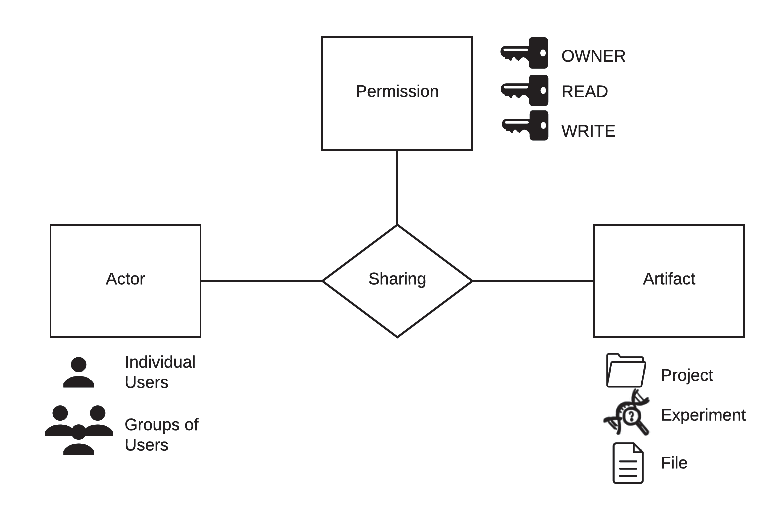
\includegraphics[height=3in, width=3.5in]{figures/sharing-concepts.pdf}
\caption{Relationship between the Actor, Permission, Artifact and Sharing concepts.}
\end{figure}\label{image:permission-model}

Actor: An Actor can either be a single user or a group of users. A group will be owned by the creator of the group and can have other users or groups as child members. Child groups can in turn have other groups, which are owned by the same owner, as child members. The implementation avoids the creation of cyclic group memberships. A particular user can be a member of a group via direct membership or via indirect membership; i.e., by being a member of another nested group or both. Based on the use cases, the direct and indirect membership can be enforced in different ways or need not be distinguished. When representing an actor we select a common metadata model that can represent individual user information as well as group information such that it can cater the usage requirements of the gateways.
Artifact: An artifact can be an arbitrary entity. A typical gateways describe artifacts to be a user project, job or a input/output file. In a more generic sense, an artifact can be any item that needs to be shared or have its access controlled. Artifacts can have hierarchical structures (i.e parent-child relationships). This hierarchy enables sharing at different granularities. For example, a user may want to share a project and all the nested child experiments and input/output files implicitly, or share only the project content without child entities. We do not allow Artifacts to have cyclic dependencies in their parent-child hierarchies. Similar to Actors, when representing Artifacts, we select a common metadata model, which includes fields such as name, description, created time, updated time, full text field and a placeholder for a binary object which can contain any type of data.
Permission: Permission defines access types that an Actor can have on an Artifact in a sharing relationship. For example, User1 may have READ permission on Experiment1, which will only grant access to view things in Experiment1. Group1 may have WRITE permission on Experiment1 which would allow a Group1 member to write/update the content in Experiment1. Sometimes it is possible that one permission may subsume the access rights defined by another permission. For instance the OWNER permission (granted to the owner of an artifact) subsumes the access rights enforced by READ and WRITE permissions, thus defined as a super permission of both READ and WRITE permissions. A particular user may have READ permission either because the item is explicitly shared with READ permission or the user has another permission (e.g. OWNER) which subsumes the access rights of the READ permission. These kinds of relationships are captured in the form of a permission hierarchy. Similar to Actors and Artifacts these hierarchies also cannot have cyclic parent-child dependencies.

\section{Implementation}
To realize the science gateway use cases summarized in Table 1, we implemented the architecture discussed above. The relationships between entities guided us to select a relational database engine. The choice of the Object-Relational Mapping enables the underlying databases such as Derby and MySQL to be plugged in seamlessly to Apache Airavata. To simplify the implementation, individual Users are treated a special type of Group with a restriction to have one member. 

Sample Scenario: We describe the sharing implementation using a hypothetical sample scenario. Let's say three users would like to define three permission types (OWNER, READ and WRITE), and collaborate on artifact types (PROJECT, EXPERIMENT, and FILE). User1 owns one project (Project1) in which contain two experiments (Experiment 1 and 2) each with an a file collection (File 1 and 2). User1 creates a parent group (Group 1) and a nested child group (Group 2). We will now walk through all 4 gateway use cases for this scenario.

\begin{figure}
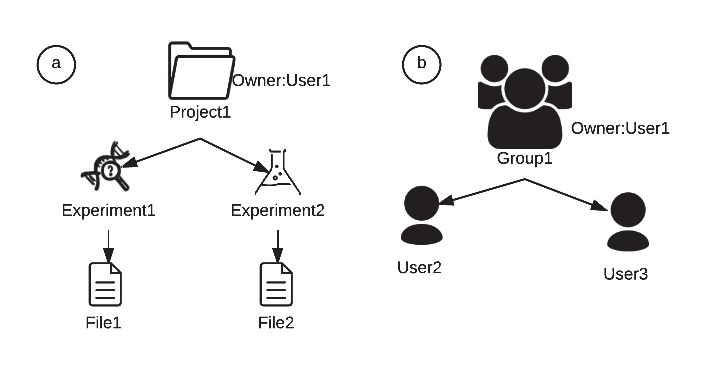
\includegraphics[width=\columnwidth]{figures/usage-scenarios.pdf}
\caption{Hypothetical user collaboration scenario. (a) Artifact hierarchy owned by User1 and (b) Group hierarchy created by User1.}
\end{figure}

Sharing and Revoking: Initially only User1 has access to Project1 and all other nested artifacts (through the default assignment of the OWNER permission). If User1 wants to give READ permission to Project1 for User2, the lucid design facilities gateways to accomplish it in multiple ways. The most basic approach would be to explicitly share Project1 with User2 with READ permission. This operation corresponds to creating an entry in Sharing table which can be represented as: 

\begin{lstlisting} 
INSERT INTO SHARING(ACTOR, ARTIFACT, PERMISSION) VALUES(User2, Project1, READ)
\end{lstlisting}

However this will allow User2 to READ Project1 and not any of its nested artifacts. If User2 also needs to have READ permission to all nested artifacts of Project1 we need to define sharing rules for all the nested artifacts rooted at Project1, either explicitly or implicitly. The implicit way to handle this is to add an additional field in the Sharing rule to capture this information. The explicit way to handle this is to traverse through the Artifact subtree and create sharing records for each nested Artifact. The two approaches can be represented as follows:

\begin{lstlisting} 
INSERT INTO SHARING(ACTOR, ARTIFACT, PERMISSION, CASCADE) VALUES(User2,Project1, READ, True)
\end{lstlisting}

\begin{lstlisting} 
Q := Queue()
Q.dequeue(Project1)
While NOT Q.empty()
  X := Q.dequeue()
  INSERT INTO SHARING(ACTOR, ARTIFACT, PERMISSION, CASCADE) VALUES(User2, X, READ, True)
  Q.enqueueAll(X.getChildren())
\end{lstlisting}

There are tradeoffs in choosing between these two approaches. The implicit approach has constant time complexity at sharing time but requires complex and computationally expensive retrieval operations at inference time (i.e Check permission and Search operations). On the other hand, the explicit approach has O(n) time complexity (n is the number of artifacts in the subtree) and requires constant time complexity at inference time. In a practical setting, most operations the sharing model should support will be inference type operations. Hence in our model we have decided to use the explicit approach.

To explain the need for CASCADE field, consider the following case. Assume that User1 has shared Project1 and all its child Artifacts granting User2 READ permission. Later User1 creates a new Experiment (Experiment 3) which is nested under Project1. User2 should have READ access to the new Experiment 3, even though it is created after Project1 was shared. To achieve this, Experiment 3 should inherit all the Sharing rules from its parent that  are cascadable at creation time. To determine whether a sharing rule is cascadable we maintain a CASCADE field in the Sharing rule.

\begin{lstlisting}
Parent := Experiment3.getParent()
SharingRules := SELECT * FROM SHARING WHERE SHARING.ARTIFACT = Parent AND  SHARING.CASCADE = True
For Rule in SharingRules
  INSERT INTO SHARING(ACTOR, ARTIFACT, PERMISSION, CASCADE) VALUES(Rule.ACTOR, Experiment3, Rule.PERMISSION, True)
\end{lstlisting}

The model also provides the capability to revoke already defined sharing rules. This operation corresponds to the deletion of the specific Sharing rule. But some complications may arise in the case of cascading sharing rules when multiple inheritance yields the same Permission. For example, assume Experiment 1 and its child artifacts are shared with User2 with READ permission. This allows User2 to READ the File1. The corresponding entry in the Sharing can be written as:

\begin{lstlisting}
INSERT INTO SHARING(ACTOR, ARTIFACT, PERMISSION, CASCADE) VALUES(User2, File1, READ, True)
\end{lstlisting}

If User1 later decides to Share the Project1 and all its child artifacts with User2 with READ permission, this Sharing rule will also enable User2 to READ File1. But note that the corresponding Sharing rule entry for Experiment1 and File1 will be the same as in the previous case. This will either duplicate the Sharing rule or would not make any changes, based on the implementation. Later if User1 wants to revoke the Sharing defined on Experiment1, all the Sharing rules that were created as a result of that Sharing have to be deleted as per the following operation.

\begin{lstlisting}
Q := Queue()
Q.dequeue(Project1)
While NOT Q.empty()
  X := Q.dequeue()
  DELETE FROM SHARING WHERE SHARING.ACTOR = User2 AND SHARING.PERMISSION = READ
  Q.enqueueAll(X.getChildren())
\end{lstlisting}

This will end up having only one Sharing rule allowing User2 to READ and Project1 and nothing else. Hence it is important to capture the inheriting parent Artifact when recording cascading Sharing rules and at the revocation time deleting only the ones that correspond to the specific revoking parent Artifact. The modified Sharing operation on Project1 will now look as follows.

\begin{lstlisting}
Q := Queue()
Q.enqueue(Project1)
While NOT Q.empty()
  X := Q.dequeue()
  INSERT INTO SHARING(ACTOR, ARTIFACT, PERMISSION, CASCADE, INHERITING_SUPER_PARENT) VALUES(User2, X, READ, True, Project1)
  Q.enqueueAll(X.getChildren())
\end{lstlisting}

Going back to our first scenario, granting User2 with READ permission on Project1, we could have achieved this in two other ways. One approach would be to use the Permission type hierarchy and Share Project1 with a Super permission of READ (e.g). An actor who has OWNER Permission on an Artifact will also have READ Permission. The other approach would be to Share the Artifact with an Actor that contains the User2. For example if Project1 is Shared with Group1 with READ Permission, then User2 will also have READ Permission on Project1 as a result of being a member of Group1. Similar to handling nested hierarchies in Artifacts, the nested hierarchies in Permission types and Groups can be handled either implicitly or explicitly. The implicit approach will record only the original Sharing rule and will defer the heavy lifting to the inference time. On the other hand, in the explicit approach, addition records will be created to each nested element. For example when Sharing with OWNER permission additional records will be created to READ and WRITE permission. However we found that most of the Permission Type and Group hierarchies in our use cases are short and flat and always will be of cascade type (e.g. when sharing with a group it is always implied that it is sharing with all the nested members). Therefore the overhead of using the implicit approach is not significant. Hence we use the implicit approach to handle Permission type and Group hierarchies.

Check Permissions: In our model, inference operations become straightforward and less costly because we put most of the computational heavy lifting on the sharing and revoking operations. The Check Permissions operation determines whether a specific Actor has a specific Permission to a specific Artifact. For example, consider the case where we want to determine whether User2 has READ Permission to Project1. In our model, which implicitly captures nested aspects in Permissions and Groups, we need to first find all the Permissions which subsume the READ permission and all groups that have User2 as a member. After finding those, Check Permissions can be easily executed as follows.

\begin{lstlisting}
Groups := User2.getAllMemberGroups()
Groups := Groups U User2
Permissions := READ.getSuperPermissions()
Permissions := Permissions U READ
SELECT HasPermission as Count(*) > 0 FROM SHARING WHERE SHARING.ACTOR IN Groups AND SHARING.PERMISSION IN  Permissions AND SHARING.ARTIFACT = Project1
Return HasPermission
\end{lstlisting}

Get all Accessible Actors: Sometimes it is useful to view a list of Actors who have Permission to READ or WRITE an Artifact. For example, the Owner of an Artifact may want to review the current list of Actors before granting or revoking sharing permissions. To get the list of Actors we create a relational join between Actors and Sharing entities and then use a filter operation to retrieve the list of Actors who have a particular Permission to an Artifact. For example, the operation to find out the list of Actors who has READ permission to Experiment 1 can be executed as follows:

\begin{lstlisting}
Permissions := READ.getSuperPermissions()
Permissions := Permissions U READ
SELECT ACTOR AS A FROM SHARING JOIN ACTOR WHERE SHARING.PERMISSION IN Permissions AND SHARING.ARTIFACT = Experiment1
Return A
\end{lstlisting}

Search/Browse: In the search operation, the objective is to retrieve a list of Artifacts that are accessible to a specific actor based on some permission criteria and that conforms to a particular search criteria on Artifact properties. As explained earlier, Browse is special case of search with empty Artifact filter criteria. As a practical requirement, when dealing with large return lists, it is also important to handle pagination. As the objective of this operation is to retrieve the list of Artifacts we do a relational join between Artifact and Sharing entities and then apply the filter criteria. In the current implementation, the Artifact filter criteria can be applied on Artifact name, description, owner, parent artifact (if exists), created and updated times and the full text field. Some of the example search/browse queries will be as follows:

\begin{itemize}
\item
Browse without Artifact type constraint: e.g. Select Artifacts where User2 has READ access.
\item
Browse with Artifact type constraint: e.g. Select Artifacts of type EXPERIMENT where User2 has READ access.
\item
Search with Artifact filter criteria: e.g. Select first 10 Artifacts of type EXPERIMENT where User2 has READ access and the Artifact name contains ``Ethylbenzene'' and Artifact created during last week.
\end{itemize}

The last search operation listed above can achieved as follows:

\begin{lstlisting}
Groups := User2.getAllMemberGroups()
Groups := Groups U User2
Permissions := READ.getSuperPermissions()
Permissions := Permissions U READ
SELECT ARTIFACT AS A FROM SHARING JOIN ARTIFACT WHERE SHARING.ACTOR IN Groups AND SHARING.PERMISSION IN  Permissions AND ARTIFACT.TYPE = EXPERIMENT AND ARTIFACT.NAME CONTAINS “EthylBenzene” AND ARTIFACT.CREATED_DATE IN LAST_WEEK LIMIT 10 OFFSET 0
Return A
\end{lstlisting}

\section{Integration with SEAGrid}

SEAGrid provides a traditionally secure data model where all the data has been considered to be proprietary and data sharing occurs only outside the SEAGrid application. However, recently users have requested the data be made shareable among collaborators to improve organization, post-processing and collaborative discovery. The discovery and sharing of the data go hand in hand as the simulation data accumulates over time and data location and identity need to be maintained to reuse the same in subsequent simulations. Supporting data discovery by individual users and collaborative processing of data requires both metadata generation and data indexing. The original SEAGrid infrastructure provided a way to define key value pairs so users can manually add to a metadata catalog for each experiment they set up, along with a search engine to discover the tagged data and products. However, users did not adopt this system, as it required a disciplined addition of metadata tags.  

Recently we eliminated the manual tagging operations by implementing an automated parsing and indexing system. This system generates metadata tags for output of some of the applications used in the SEAGrid gateway \cite{nakandala2016anatomy}. The parsing infrastructure created for the SEAGrid gateway provides access and discovery of any data shared with the user, as it becomes part of the searchable domain. Additional sharing infrastructure requires us to define what is shared and with whom and a way to collaboratively process data. Toward this end we have prototyped integrating Jupyter notebooks in a GSOC project that can be integrated into Apache Airavata gateway infrastructures to interact with data products with ready analysis functions available in Python \cite{xsedeGateways}.   

The users have benefitted from the job history organization already available in the portal but were unable to exploit the vast amount of past data from the community as there was no infrastructure to share the data securely. SEAGrid now provides a generic way to publish data to community organizations such as Figshare or SeedMe.org, but more controlled sharing for collaborative and cooperative post-processing will require additional infrastructure to define collaborating individuals or groups, modes of sharing, and timelines. Sharing of post-processing functions/applications along with the data and/or provenance details would also be beneficial for reproducing data products as well additional enhancement to the analysis if needed.
In addition to the data sharing requirements, SEAGrid may have to restrict resources such as applications due to accessibility to license, something that is being tested by a PI  or one  based on a restricted hardware resource such as campus/institutional  resource. The group and sharing infrastructure need to support these modalities as well. 

\section{Integration with the CIPRES Workbench Framework}\label{nsg}

The CIPRES Workbench Framework \cite{miller2015cipres} was created with the assumption that each authenticated user was working independently of all others, which is consistent with the work paradigm of biological science when the software was designed. The software at present does not support collaboration or data sharing between individual accounts. However, recent surveys show that users of the Neuroscience Gateway (NSG) and the CIPRES Science Gateway, two highly accessed gateways built using the CIPRES Workbench framework, have a strong interest in sharing data within their workgroups, and with the public as well [REF-Majumdar; Miller, unpublished data]. Both user groups indicate that data access and data sharing present a significant challenge, and that users would appreciate a solution that can be managed from within the Gateway interface. Two specific use cases highlighting the data sharing needs of typical Workbench Framework users  are listed below:

A geographically distributed, highly interdisciplinary neuroscience research group is interested in collaboration that combines empirical results from magnetoencephalography (MEG) experiments with detailed computational models of neocortical circuitry to infer the mechanisms responsible for generating cortical rhythmic activity. Experimental data is collected from geographically distributed collaborators' institutions, yet jointly all of them are developing a large-scale model of thalamocortical circuitry with detailed neurons and synaptic architectures and plan to run on supercomputers. Model predictions will be validated and informed with simultaneous thalamic and cortical microelectrode recording data (that needs to be shared) obtained in the collaborators' lab in other institutions in US and France \cite{delorme2004eeglab}. 

EEGLAB [REF-EEGLab] is a widely used software for processing experimental eletrophysiological (EEG) data by thousands of cognitive neuroscientists worldwide. Researchers are now interested in meta-analysis of source-resolved EEG measures across studies. This will allow research results of individual researchers/labs to be analyzed/compared (meta-analysis) to gain deeper understanding of brain functions at a higher level. To be able to do this researchers will need a mechanism, within NSG, where they can make their data shareable such as by tagging results that they want to share with other researchers or make it public. This will require different level of sharing capabilities. This will then allow other researchers to perform meta-analysis of research results at a higher level using computing power provided by NSG.

Based on user feedback and the use cases above, tools for sharing data between accounts  are a priority feature for CIPRES Workbench users. Accordingly, we are integrating the data sharing service with the CIPRES Workbench framework. Our approach will take a somewhat different strategy from the SEAGrid integration described above. A schematic is shown in Figure 4. For the Workbench Framework, a separate group management server will allow users to perform group and user management. This will allow full access to all group/user management functions in the SciGaP sharing service without requiring any User Interface development. The CIPRES Workbench will retain an internal representation of Experiment configuration, so the shared Entities will be project folders.  Within the Workbench code, project folder identifiers will be used to determine user access to contained Data and Experiments (Tasks in workbench terminology). Integration with the Experiment Catalog will not be required.

In the implementation for CIPRES and NSG, users will be able to access shared folders and control access to their experiments and data through the browser interface of the respective applications. Authenticated users can configure sharing/display preferences for their account profile. Folders (Artifacts) the user creates can be configured individually for sharing with Users or Groups. The new interface will also provide users with the ability to check, set, and revoke sharing permissions on Artifacts they create. For data shared with the user, a “shared data” folder will appear in the user interface. Users can view shared Files, Experiments, and Projects. In our initial implementation, read-only Artifacts can be cloned from the shared folder, and then can be modified and resubmitted; the cloned jobs will be owned by the submitting user.

\section{Related Work}

Internet2’s Grouper \cite{grouperWebsite} is an access management system that is widely used in universities that can support most of the required features in our proposed solution. Grouper provides comprehensive and efficient group management functionalities including rule and time based group membership definitions and ability to define groups based on complex group math operations (unions, intersections and differences) that are generally beyond the simple group management requirements in gateways. Features in Grouper such roles, attributes, and permissions can be used to implement our sharing model. If implemented using Grouper, the system can easily support the sharing and revoking of Artifacts, check permission, and get all accessible users operations. However the lack of flexibility in the Grouper’s search/browse APIs hinders the system in efficiently fulfilling the search/browse operations required by the Gateways users. Search/Browse operations are an important aspect for Gateways, as we have described.

SeedMe \cite{chourasia2013seedme} is a cyberinfrastructure platform that enables seamless sharing and visualization of computer simulation outputs which runs on HPC infrastructures through a web based tool. It enables users to conveniently view and access simulation outputs. Users can create collections of data items and share publicly or with a specified group of users. In the current implementation it has a single permission level, which grants permission to shared users to view and comment on the collection. Also it lacks the ability to define reusable user groups and requires explicitly defining the list of users every time when sharing a collection.

Globus Groups \cite{globusFileSharing} can be used for access control by other Globus services, and are especially useful for file sharing. In the case of file sharing, file should first make it accessible as a Globus shared endpoint by configuring a Globus connect server. Then the owner of the file can share it with individual Globus users or Globus groups either with READ or WRITE permission. However it does not provide the functionality to create arbitrary Artifacts and share it with others.

\section{Conclusions}


%\begin{acks}
%  The authors would like to thank Dr. Yuhua Li for providing the
%  matlab code of  the \textit{BEPS} method. 
%
%  The authors would also like to thank the anonymous referees for
%  their valuable comments and helpful suggestions. The work is
%  supported by the \grantsponsor{GS501100001809}{National Natural
%    Science Foundation of
%    China}{http://dx.doi.org/10.13039/501100001809} under Grant
%  No.:~\grantnum{GS501100001809}{61273304}
%  and~\grantnum[http://www.nnsf.cn/youngscientsts]{GS501100001809}{Young
%    Scientsts' Support Program}.
%
%\end{acks}

\bibliographystyle{ACM-Reference-Format}
\bibliography{airavata-sharing-service-pearc17} 

\end{document}
